%!TEX root = ../paper.tex
In this section we present the results of the two estimators on dataset \ferdosiTwo, \baakmanTwo, \ferdosiThree, \baakmanThree, \ie the datasets that contain more than one Gaussian. 

%MSE
	The plots in \cref{fig:4:resuts:multiSphere} suggest some differences in how the two estimators handle the different components of the dataset, therefor 

\begin{table*}
	\centering
	%!TEX root = ../paper.tex

\begin{tabular}{@{}ccl*{2}{S[scientific-notation=true,round-mode=places,round-precision=3]}}
\toprule
~				&~					&~ 				& \multicolumn{2}{c}{Estimator}\\ \cmidrule{4-5}
Set 			&~					& Component		& {\mbe} 				& {\sambe}\\
\midrule
% Ferdosi 2
\hline
\ferdosiTwo 	&\legendDot{blue}	& Gaussian 1	& 1.560536961708337e-07 & 2.993178935719230e-07\\
~ 				&\legendDot{green}	& Gaussian 2	& 2.285260303722557e-09 & 8.344636264610111e-10\\
				&\legendDot{red}	& Noise 		& 2.021379766292543e-11 & 2.363141221512672e-11\\
% Ferdosi 3
\hline
\ferdosiThree	&\legendDot{blue}	& Gaussian 1	& 0.0 & 0.0\\
~ 				&\legendDot{green}	& Gaussian 2	& 0.0 & 0.0\\
~ 				&\legendDot{red}	& Gaussian 3	& 0.0 & 0.0\\
~ 				&\legendDot{orange}	& Gaussian 4	& 0.0 & 0.0\\
% Baakman 2
\hline
\baakmanTwo		&\legendDot{blue}	& Gaussian 1	& 0.0 & 0.0\\
~ 				&\legendDot{green}	& Gaussian 2	& 0.0 & 0.0\\
% Baakman 3
\hline
\baakmanThree	&\legendDot{blue}	& Gaussian 1 	& 0.0 & 0.0 \\
~ 				&\legendDot{green}	& Gaussian 2 	& 0.0 & 0.0 \\
~ 				&\legendDot{red}	& Gaussian 3 	& 0.0 & 0.0 \\
~ 				&\legendDot{orange}	& Gaussian 4 	& 0.0 & 0.0 \\
\bottomrule
\end{tabular}
	\caption{The mean squared error of the known densities and the densities estimated by the Modified Breiman Estimator (\mbe) and the shape-adaptive MBE (\sambe), respectively, for the Gaussian components of the datasets with multiple Gaussians.} 	
	\label{tab:4:results:mse}
\end{table*}

	\todo[inline]{Mention MSE results}
	\todo[inline]{MSE for the different components}

% PLOTS
	\begin{figure*}
		\centering
		%!TEX root = ../paper.tex

% Ferdosi 2, MBE
\begin{subfigure}{0.23\textwidth}
	\centering
	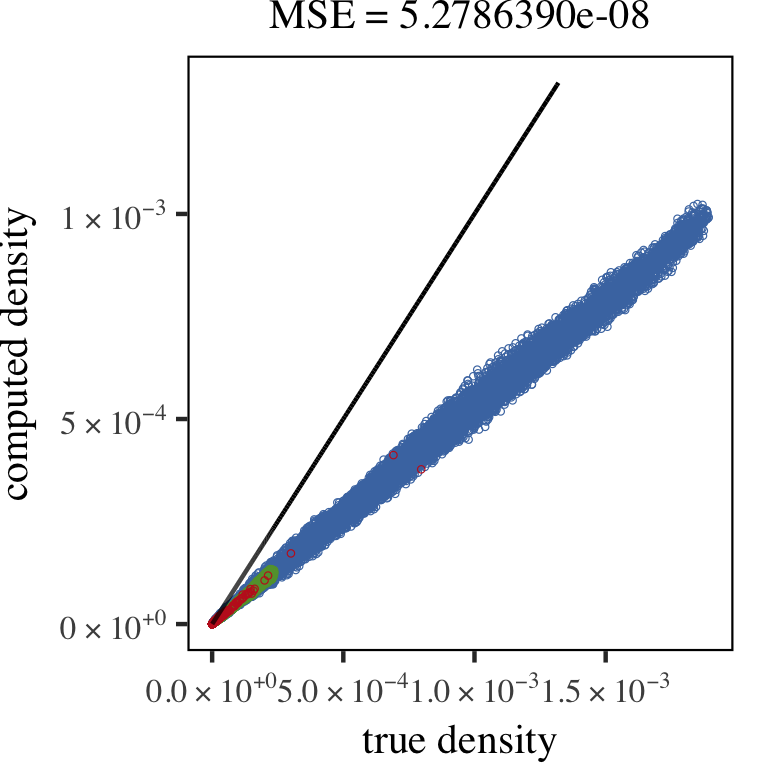
\includegraphics[keepaspectratio=true, width=\textwidth, height=0.23\textheight]{result/img/all/results_ferdosi_2_60000_mbe_silverman}
	\caption{Set \ferdosiTwo, \mbe}
	\label{fig:4:results:mbe:ferdosi2}
\end{subfigure}
% Baakman 2, MBE
\begin{subfigure}{0.23\textwidth}
	\centering
	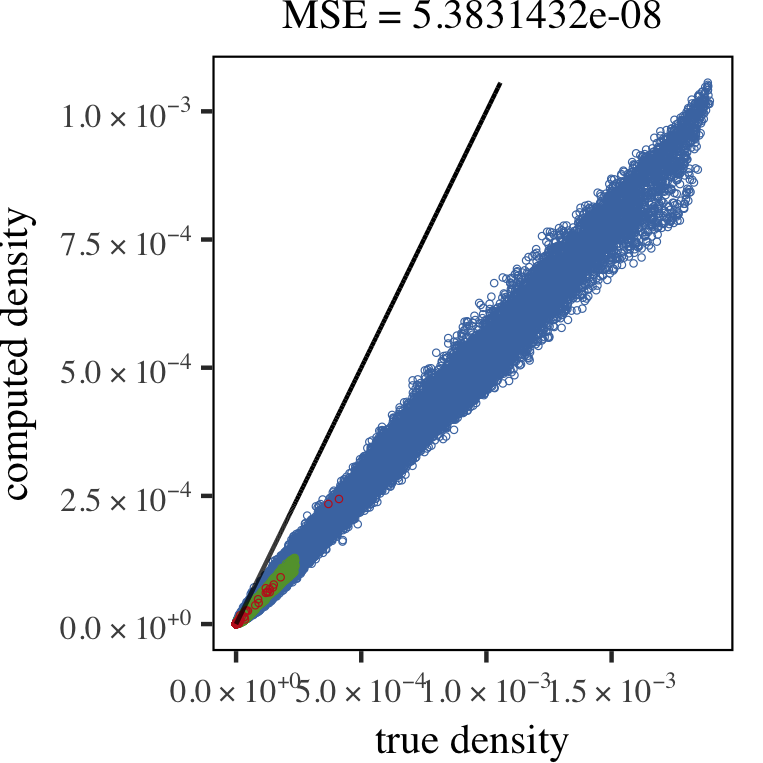
\includegraphics[keepaspectratio=true, width=\textwidth, height=0.23\textheight]{result/img/all/results_baakman_2_60000_mbe_silverman}
	\caption{Set \baakmanTwo, \mbe}
	\label{fig:4:results:mbe:baakman2}
\end{subfigure}
% Ferdosi 3, MBE
\begin{subfigure}{0.23\textwidth}
	\centering
	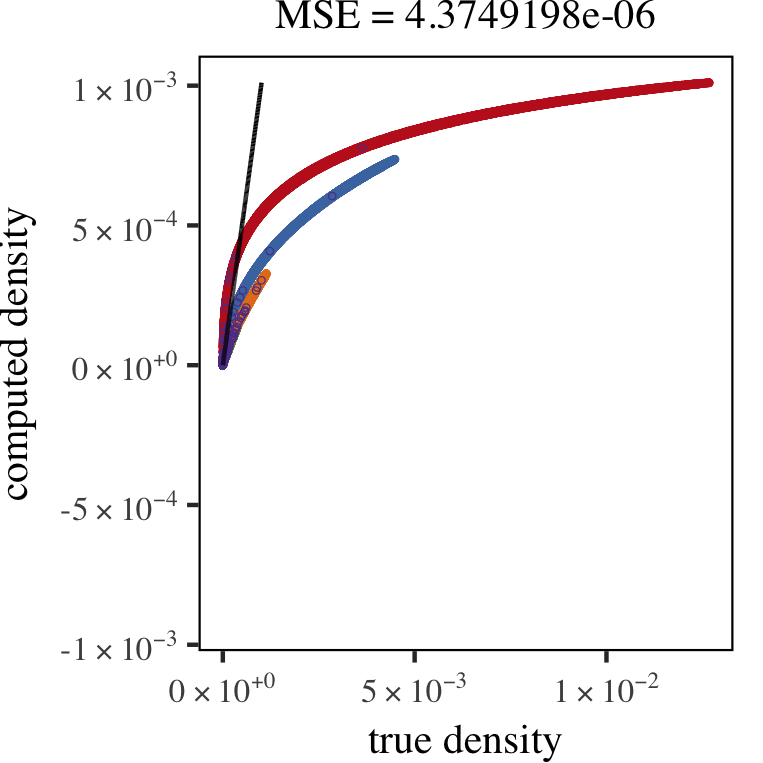
\includegraphics[keepaspectratio=true, width=\textwidth, height=0.23\textheight]{result/img/all/results_ferdosi_3_120000_mbe_silverman.png}
	\caption{Set \ferdosiThree, \mbe}
	\label{fig:4:results:mbe:ferdosi3}
\end{subfigure}
% Baakman 3, MBE
\begin{subfigure}{0.23\textwidth}
	\centering
	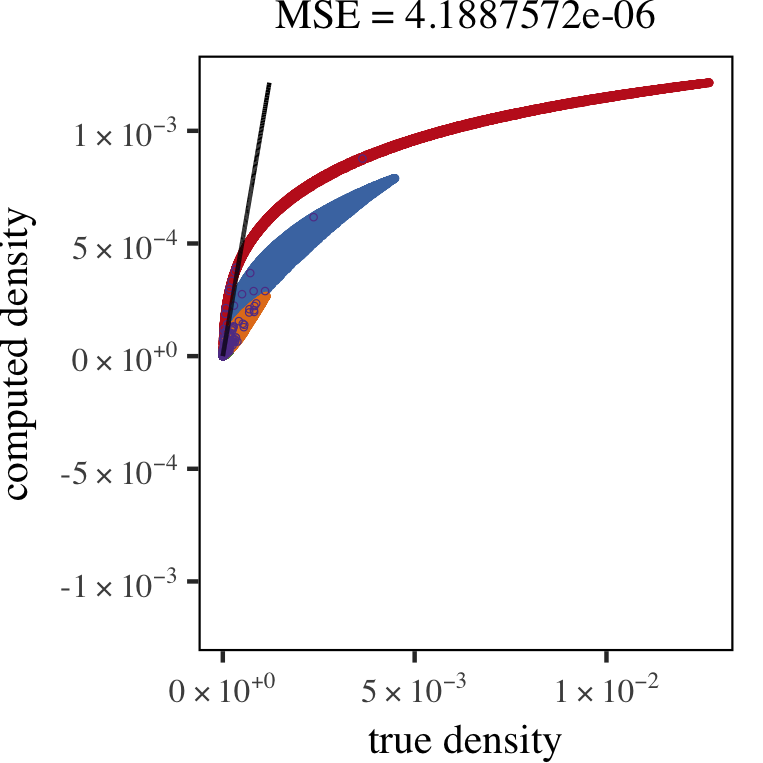
\includegraphics[keepaspectratio=true, width=\textwidth, height=0.23\textheight]{result/img/all/results_baakman_3_120000_mbe_silverman}
	\caption{Set \baakmanThree, \mbe}
	\label{fig:4:results:mbe:baakman3}
\end{subfigure}	
% Ferdosi 2, SAMBE
\begin{subfigure}{0.23\textwidth}
	\centering
	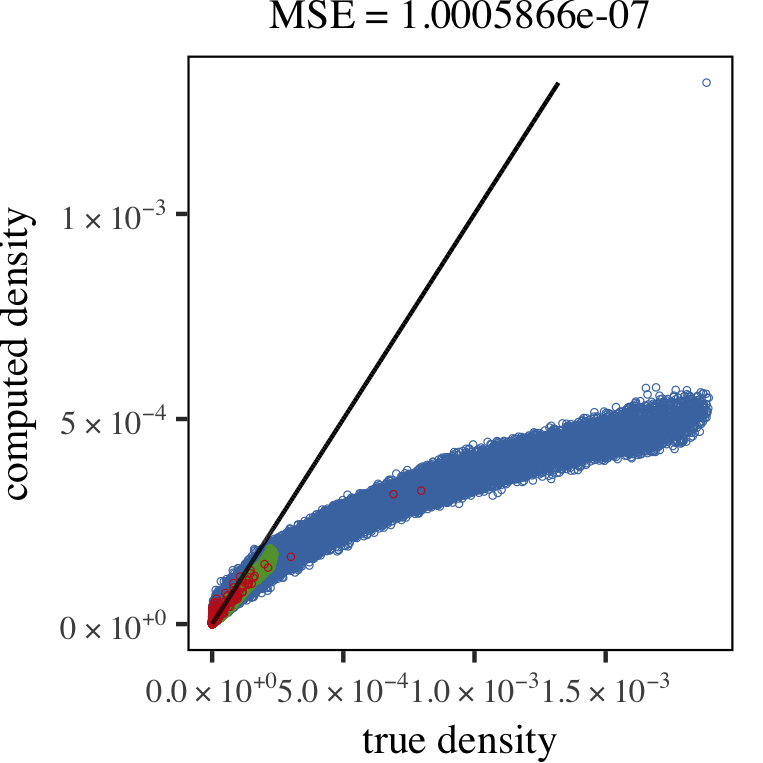
\includegraphics[keepaspectratio=true, width=\textwidth, height=0.23\textheight]{result/img/all/results_ferdosi_2_60000_sambe_silverman}
	\caption{Set \ferdosiTwo, \sambe}
	\label{fig:4:results:sambe:ferdosi2}
\end{subfigure}
% Baakman 2, SAMBE
\begin{subfigure}{0.23\textwidth}
	\centering
	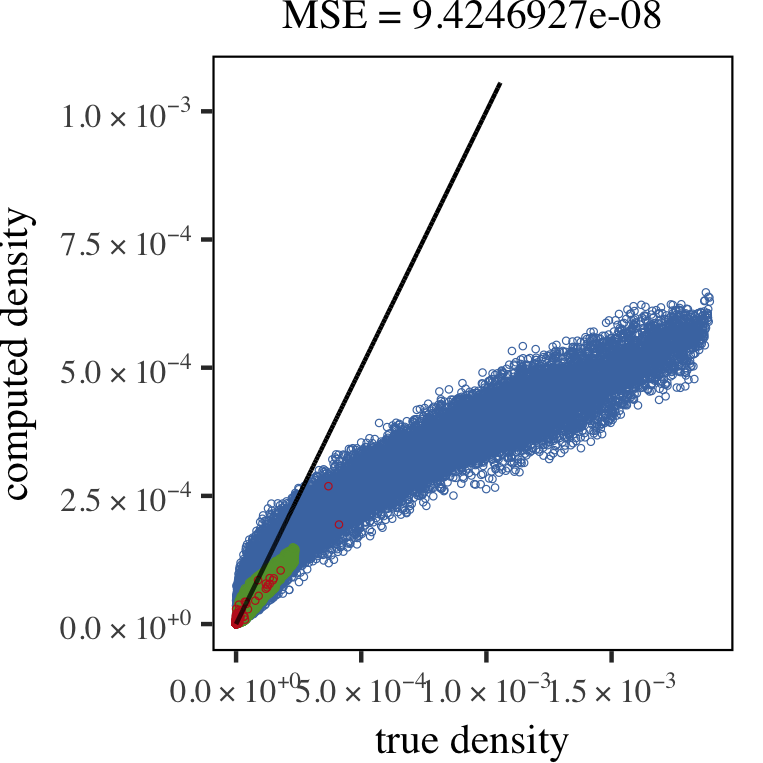
\includegraphics[keepaspectratio=true, width=\textwidth, height=0.23\textheight]{result/img/all/results_baakman_2_60000_sambe_silverman}
	\caption{Set \baakmanTwo, \sambe}
	\label{fig:4:simulated:datasets:sambe:baakman2}
\end{subfigure}
% Ferdosi 3, SAMBE
\begin{subfigure}{0.23\textwidth}
	\centering
	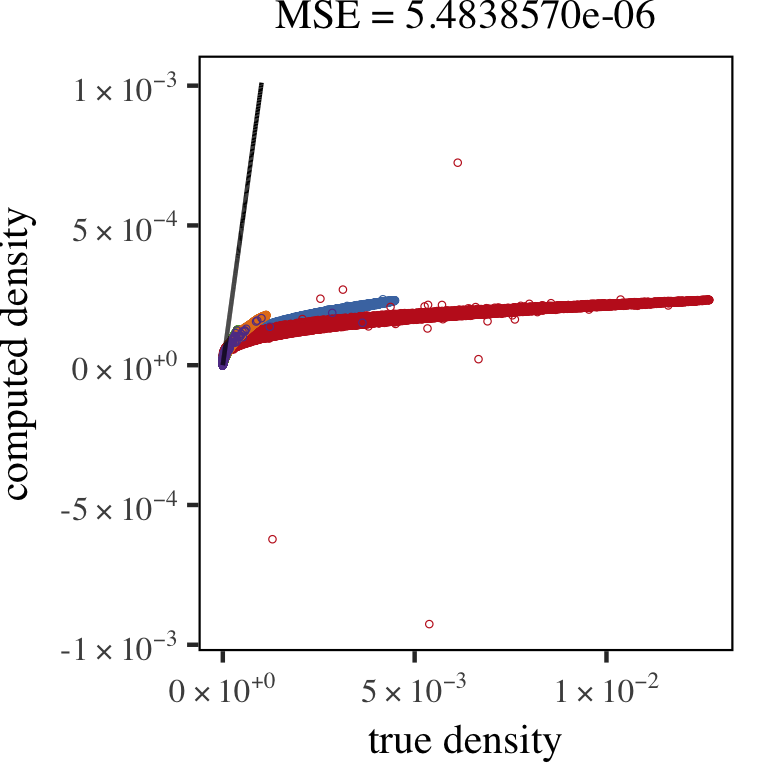
\includegraphics[keepaspectratio=true, width=\textwidth, height=0.23\textheight]{result/img/all/results_ferdosi_3_120000_sambe_silverman}
	\caption{Set \ferdosiThree, \sambe}
	\label{fig:4:simulated:datasets:sambe:ferdosi3}
\end{subfigure}
% Baakman 3, SAMBE
\begin{subfigure}{0.23\textwidth}
	\centering
	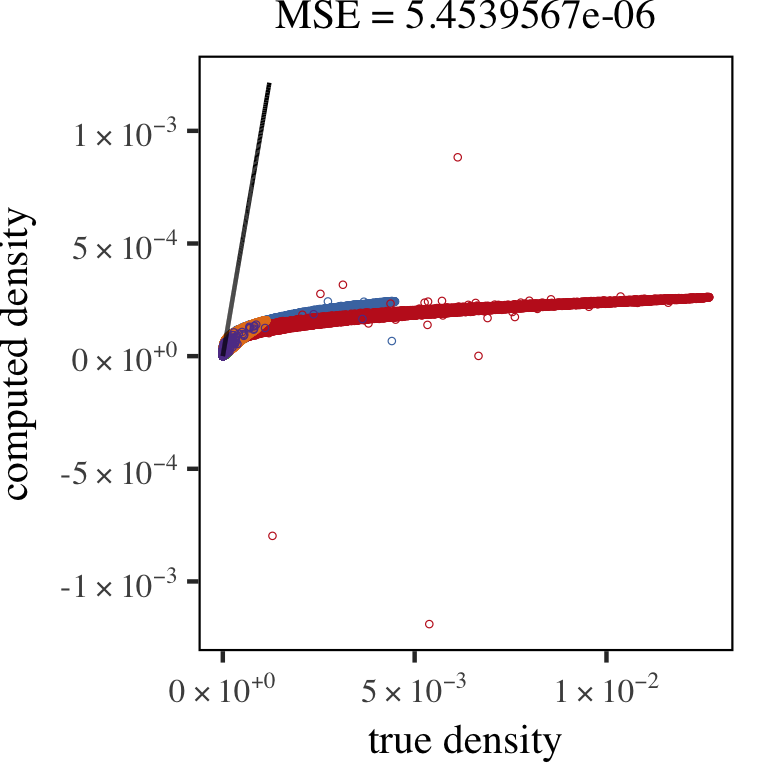
\includegraphics[keepaspectratio=true, width=\textwidth, height=0.23\textheight]{result/img/all/results_baakman_3_120000_sambe_silverman}
	\caption{Set \baakmanThree, \sambe}
	\label{fig:4:results:sambe:baakman3}
\end{subfigure}	
		\caption{Comparative plots for dataset \ferdosiTwoNum, \ferdosiThreeNum, \baakmanTwoNum, and \baakmanThreeNum.}
		\label{fig:4:resuts:multiSphere}
	\end{figure*}

	\todo[inline]{Point to \cref{fig:4:resuts:multiSphere}}.
	\todo[inline]{Report on \cref{fig:4:results:mbe:ferdosi2} and \cref{fig:4:results:mbe:baakman2}.} 
	\todo[inline]{Report on \cref{fig:4:results:mbe:ferdosi3} and \cref{fig:4:results:mbe:baakman3}.}

	\todo[inline]{General observation of multi sphere datasets.}